\documentclass[conference]{IEEEtran}

\IEEEoverridecommandlockouts

\usepackage{cite}
\usepackage{amsmath,amssymb,amsfonts}
\usepackage{algorithmic}
\usepackage{graphicx}
\usepackage{textcomp}
\usepackage{xcolor}

\def\BibTeX{{\rm B\kern-.05em{\sc i\kern-.025em b}\kern-.08em
    T\kern-.1667em\lower.7ex\hbox{E}\kern-.125emX}}
\begin{document}

\title{Streaming via HTTP3: is it better, and how do we start it as QUICkly as possible?}

\author{\IEEEauthorblockN{1\textsuperscript{st} Nick Lehmann}
  \IEEEauthorblockA{
    \textit{TU Dresden}\\
    Dresden, Germany \\
    nick.lehmann@mailbox.tu-dresden.de
  }
}

\maketitle

\begin{abstract}
This paper investigates the performance of QUIC, a protocol originally announced and developed by Google. QUIC was standardized in 2019 and is now the basis for HTTP/3. We have a look at the performance of QUIC by collecting performance results from different papers and explain why results from different researchers can vary significantly. The result is an overall comparison of QUIC to HTTP/1 and HTTP/2 where we emphasize how QUIC achieves better startup times.
\end{abstract}

\begin{IEEEkeywords}
QUIC, HTTP, Performance
\end{IEEEkeywords}

\section{Introduction}

QUIC serves as a replacement for the network protocols that were the foundation for previous versions of HTTP. It replaces TCP by implementing a reliable connection on top of the otherwise unreliable UDP protocol. Furthermore, it replaces TLS with its encryption algorithm that allows for faster connection buildup. QUIC is often used as a synonym for HTTP/3, but it is not the case. However, since QUIC was designed and is exclusively used for HTTP/3, both terms are often used interchangeably. Strictly speaking, HTTP/3 is a reformulation of the widespread HTTP concepts on top of QUIC.

In contrast to HTTP/1, where streaming was done using workarounds on top of an otherwise request-response-oriented protocol, QUIC was developed with streaming at its core. Streams are now the native concept and single requests are modeled on top of the streams.

As this paper aims to evaluate streaming, we have to first clarify what is exactly meant by this term. From the perspective of the QUIC transport layer, everything transport of bytes is a stream. However, a developer working with HTTP/3, an application layer built on top of QUIC, would differentiate between classical requests and responses on one side (which are realized using QUIC streams), and HTTP streaming on the other side. Typical examples of the latter are video players or conferencing tools where the next seconds of the video and audio are streamed to the client, either on-demand or as soon as they become available.

This paper does not conduct any new experiments. Instead, we collect results from different papers released between 2016 and 2021 and compare them. Furthermore, we explain how QUIC has changed over the years to put the results from different times into context and to explain why some differ significantly from each other.

% Earlier papers only focused on gQUIC; first search results as they were cited more often

\section{History}

\subsection{HTTP/1}
% 1995

HTTP/1 is a request-response-oriented protocol. The client can send an arbitrary amount of requests to a server, which in return sends back a single response for each request made. This model was fine for the early days of the world-wide-web when all websites were static. 

Typically, a browser installed on the user's machine acts as the HTTP client. If the user decides to visit a website, the browser would send a GET request to the server, which in return responds with an HTML document. While a pure HTML document can be enough to completely display a website, many websites need more assets to be displayed correctly. These assets often include images as well as Javascript and CSS files.

Upon receiving the HTTP document, the browser can then build up additional TCP connections to fetch every individual asset needed to render the website. While this is a robust mechanism, it leaves a significant amount of performance on the table.

% Limit to open TCP connections becomes the bottleneck
TCP connections require the host to save some session state. Therefore, both clients and servers usually restrict the number of TCP connections that can be open at any time. This can further increase page loading time when a multitude of assets has to be fetched from the server \cite{HowQuickIsQuic}. 

% pipeline failed as a workaround because of deployment issues

% forces developers to concatenate CSS and Javascript files which hinders caching and delays processing 
To work against the costs of fetching many small files from a server using TCP, developers started to bundle many assets into single files. However, this approach comes with a few disadvantages. Firstly, it adds a step and additional complexity to the development workflow. It also hinders caching.

\subsection{HTTP/2 (SPDY)}

% History
In 2009, Google announced to work on a new network protocol called SPDY which was then deployed in 2010. Google tried to fix the issues mentioned with HTTP/1.

% Streaming
In contrast to HTTP/1, SPDY opens only a single TCP connection to the server. After that, it uses its framing layer to multiplex multiple requests over this single connection. These requests form bidirectional streams inside the connections. In addition, the server gained the ability to open streams too \cite{HowQuickIsQuic}.

% Request prioritization
Another feature of SPDY was request prioritization. Clients could specify a priority level for each stream and the server then schedules the data transfer to send the objects with the highest prioritization first. Hence, browsers were able to prioritize resources needed for rendering the page, e.g., Javascript code, while images outside of the initial viewport receive a lower priority \cite{HowQuickIsQuic}.

% Header compression
Many websites require many subrequests after the initial page has loaded. In HTTP/1, the client has to send all required HTTP headers again with each request. Therefore, SPDY introduces a header compression to reduce the number of bytes that must be transmitted.

% Server push
In some cases, the server might already know which resources the client will likely request next. Using the new server push mechanism, the server can send these objects preemptively to the client. However, the server does not know which objects are already in the client's cache, and many objects transmitted using a server push were often unnecessary. Hence, the mechanism was not used to a great extent and Chromium has removed support for it \cite{RemoveServerPush}.

% RFC
% TODO

% Performance
The performance of SPDY is still under discussion. If SPDY outperforms HTTP/1 depends on the parameters of the underlying network link. The results of most studies can be summarised by the following findings.

\begin{itemize}
  \item SPDY outperforms HTTP when the object count and RTT are high due to multiplexing and header compression
  \item SPDY performs better when the bandwidth is low
  \item HTTP performance degrades less when the package loss increases compared to SPDY
\end{itemize}


\section{QUIC}

% HTTP/3 uses the same semantics as the earlier revisions, including the same request methods, status codes, and message fields, but encodes them differently and maintains session state differently. 
% Implemented completely in userspace to allow for faster iterations during its early development. 
The introduction of a new network protocol is a very complex process. To prove that a new network protocol is an improvement over the status quo, researchers often create a reference implementation used to carry out real-world experiments. To facilitate the deployments of the QUIC reference implementations, its authors opted to use UDP as the underlying layer three protocol. UDP is not used as often as TCP but virtually every operating system supports it.

% However, there is no reason why QUIC could not become part of the Linux kernel, as well as other kernels. 
UDP is a simple protocol that has no concept of a point-to-point connection and provides no guarantees. QUIC builds on top of this unreliable protocol. Current QUIC implementations run completely in userspace. This reduced the time for the prototype and increased the speed with which the author iterated on QUIC. In contrast, kernel-space implementations are faster due to fewer context switches. In May 2022, QUIC did not land in the Linux kernel just yet, but some researchers have already implemented and evaluated QUIC in the Linux kernel \cite{Kernel}.

% TCP HOL
% UPD was chosen as it is supported on virtually every host and is very minimal. QUIC is implemented on top.
While TCP has served its users well over the last decades, it has some serious design flaws. Head-of-line blocking (HOL) can occur in two different places in HTTP/1.



\subsection{Streaming and Multiplexing}
% Streams are native concept; request-response model implemented on top

Streams are the fundamental concept of QUIC. After the client and server establish a connection, every participant can start a stream, send data over it, and close the stream at any time. 

To multiplex multiple streams over a single connection, an identifier is included in every stream frame.

Participants communicate by exchanging UDP datagrams which can contain multiple QUIC packets. Most of the QUIC packets contain frames of which there are several types. Each frame includes data associated with a single stream.

Similar to TCP, QUIC ensures the byte order, but only for a single stream and not between multiple streams.

\subsection{Encryption}

\begin{figure}[htbp]
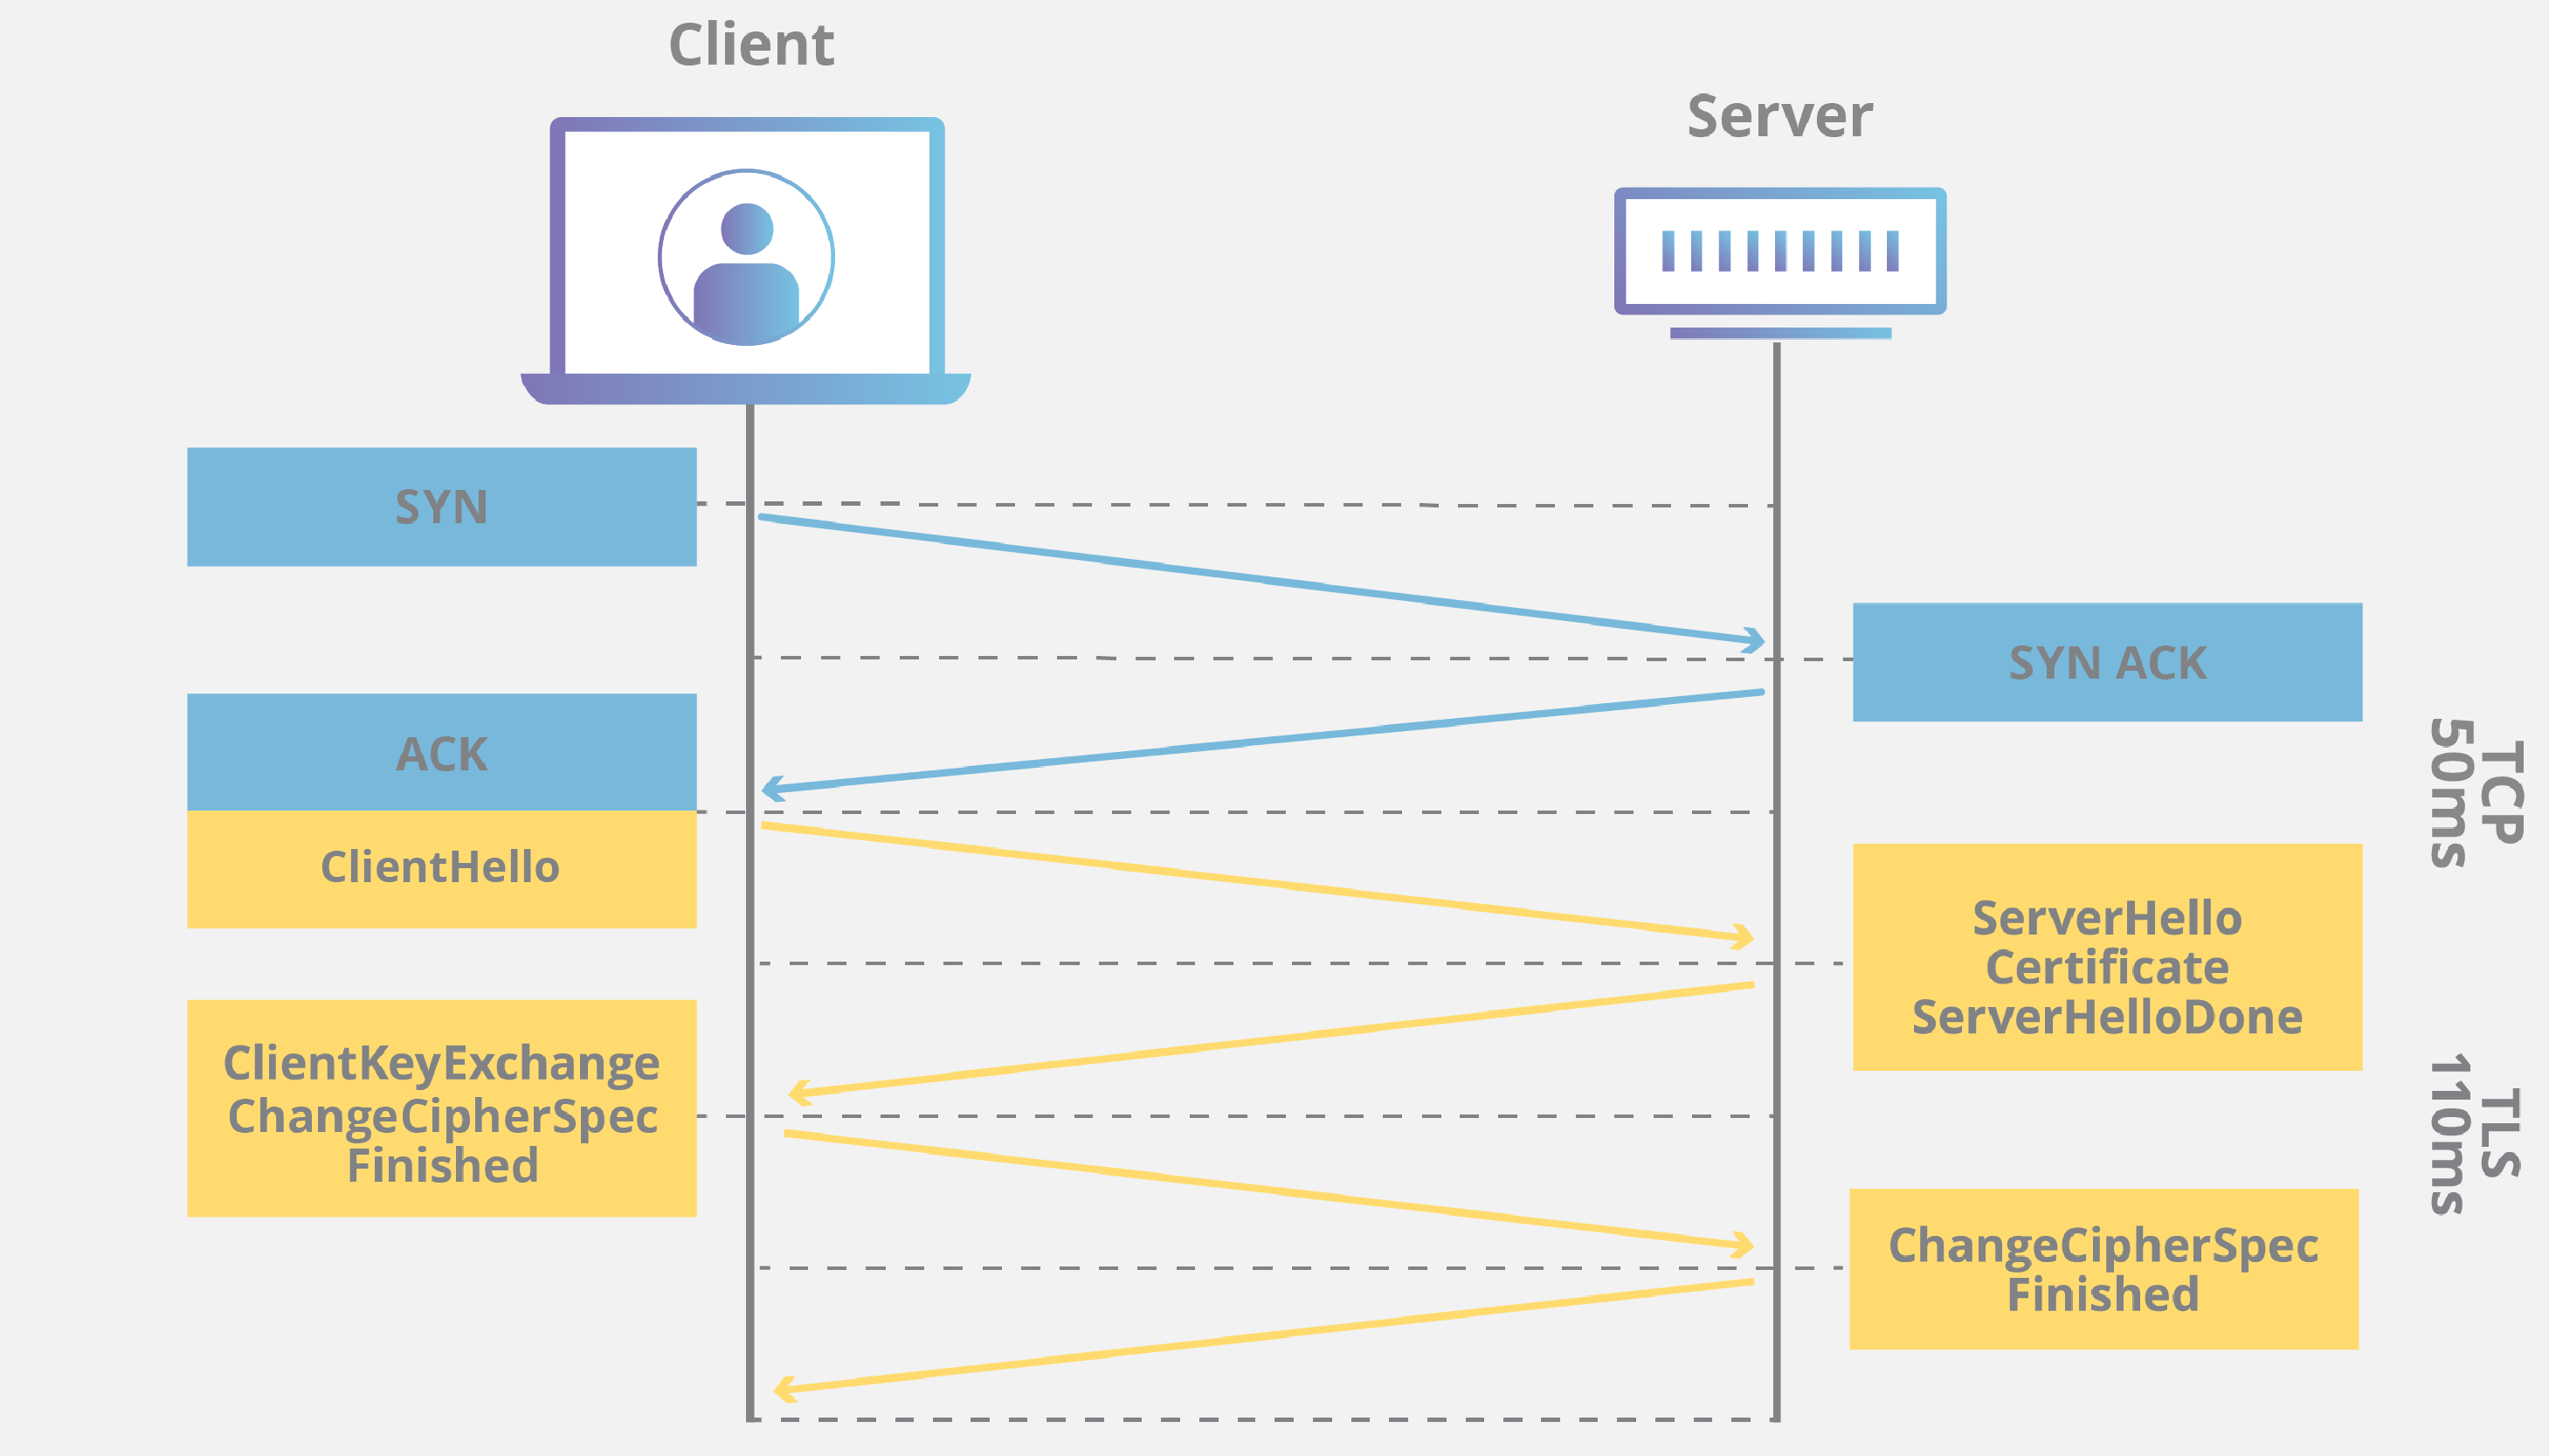
\includegraphics[width=8cm,keepaspectratio]{images/TLS handshake.png}
\caption{TLS handshake \cite{CloudflareTlsHandshake}}
\label{fig:tls-handshake}
\end{figure}

% Replaces SSL/TLS
QUIC introduces a new encryption mechanism that replaces TLS. Figure \ref{fig:tls-handshake} shows the step involved in a TLS handshake. QUIC's encryption mechanism reduces the round trips required to establish a secure connection between client and server while its safety remains comparable to TLS. Its design resembles the Datagram Transport Layer Security \cite{HowQuickIsQuic}.

\subsection{0RTT and 1RTT}
% Connection ID included in every packet.
QUIC includes a connection ID in every packet. This identifier replaces the traditional IP four-tuple, which consists of the source and destination IP address and their corresponding ports.

% Used to cache parameters for connection when there has already been a connection between client and server.
A pair of client and server can use the connection ID to cache the security parameters when they established the first secure connection between each other. A client can then utilize the cached parameters in future connections. Instead of negotiating the parameters again, it can immediately send data in the first packet, allowing for a 0RTT connection buildup.

% Connection IDs also allow for a fast resume of the connection after the client changes the network interface. 
Connection IDs have the additional benefit that they are independent of the IP address assigned to them by an internet service provider. It is common for mobile clients, e.g. cell phones, to physically move from the service area of a broadcast tower to the service area of the next one. By doing so, the mobile client usually receives a new IP address and has to inform the server of the new address to resume the connection. The usage of an address-independent connection identifier greatly simplifies these handovers \cite{HowQuickIsQuic}.

% Connection for the first time -> first request sent over TCP to negotiate if server speaks QUIC.
It is worth noting, that the 0RTT and 1RTT mechanisms of QUIC are only available if the client already knows that the server can speak QUIC. If the client does not know this in advance, it uses TCP and TLS for the connection. As stated in \cite{Google}, the server will then respond with an \textit{Alt-Svc} header in the HTTP response. After receiving the header, the client can attempt to establish a connection using QUIC. On subsequent HTTP requests, the client will try QUIC immediately. However, if the connection buildup fails or no packet is received within 300ms, the client will fall back to TCP and TLS.

% Mobile applications might already know if the server speaks QUIC or not
The drawback, that the first connection to a server has to be TCP, can be remedied in mobile applications as they often know which server they are going to talk to. For example, the YouTube app was one of the applications used by Google for testing QUIC. As both server and client are controlled by Google, they could skip the initial TCP connection. However, even in these cases, the application might have to fall back to TCP, as some routers block UDP, blocking QUIC altogether.

% \subsection{Congestion control algorithm, Hybrid Slow Start}
\subsection{Congestion control algorithm}

% TCP-Cubic by default
Similar to TCP, QUIC can be used with different congestion control algorithms. In the early implementations, QUIC used Cubic by default. However, Reno and the Bottleneck Bandwidth and Round-trip propagation time (BBR) algorithm are two other popular choices.

% Improved inputs for the congestion control algorithms
All these congestion control algorithms are not new and have been used with TCP for a very long time. However, QUIC provides more precise inputs for these algorithms to work with. Its new ACK implementation eliminates ACK ambiguity which occurs when TCP cannot differentiate between lost packets and out-of-order delivery. Together with more precise timing information, the existing algorithms might be able to perform better when used together with QUIC instead of TCP.

% Fairness
QUIC uses existing congestion control algorithms but configures them differently. Due to its multiplexing nature, a single QUIC connection effectively emulates multiple TCP connections. Hence, some researchers investigated if both protocols behave fairly when they concurrently use the same link. While \cite{Yu} reports that TCP dramatically grabs more of the bandwidth of the shared link compared to QUIC, \cite{Kakhki} observes the exact opposite. However, most of the experiments we look at in this work are tested individually and since the fairness of QUIC does not help us to study if it can start up faster, we do not investigate it further.

% A single QUIC connection is equivalent to multiple TCP connections. The congestion control algorithm can be configured to be similarly aggressive as multiple TCP connections.
% - TCP outperforms QUIC when they compete \cite{Yu}
% - QUIC outperforms TCP when they compete \cite{Kakhki}

% \subsection{Flow control}
% Flow control protects the receiver from getting overwhelmed by a very fast sender. Receivers only have a limited amount of memory to store data that was not already acknowledged.
% Receivers advertises both the limit of total bytes per stream and per connection \cite[Section 4.1]{RFC}. 

% \subsection{Packet sizing}
% 

\subsection{Forward Error Correction (FEC)}
% Proactive speculative retransmission of important packets.
% Many early papers talk about this mechanism. Turned out to be harmful to performance. Canceled for version one but research topic for the second version.

QUIC tried to decrease the latency of a connection through a technique called forward error correction (FEC). It speculated proactively which critical packets might get lost and retransmits them without waiting for a notification from the receiver. As a side effect, this would decrease the effective bandwidth of the link as data that was successfully sent after all gets transmitted twice. However, the authors of QUIC were willing to make this trade-off. 

Many of the earlier papers about QUIC investigated the effects of FEC \cite{HTTPoverUDP}. They concluded that FEC negatively impacted the performance of QUIC. FEC was then removed from the roadmap for QUIC version one. Therefore, later papers ignore FEC altogether.

When the flaws of the first implementation of FEC are fixed, this mechanism could decrease the time needed to start a QUIC stream even further. If the client speculates that the initial packet gets lost on the link, it could retransmit it without it waiting for another round trip for a notification. Due to the congestion control, QUIC is not likely to saturate the link at the beginning of the connection. Hence, transmitting a packet twice might not be noticeable.


\section{Performance}
\label{sec:Performance}

QUIC was announced in 2013 by Google and since that, many researchers have tested the potential performance advantages compared to HTTP/1 and HTTP/2. As already mentioned, QUIC was implemented completely in user space to allow for rapid development iteration. While this allowed to easily change parts of QUIC, it also brings the disadvantage that the findings of papers are only valid for a certain point in time. In contrast, the TCP stack in Linux, the dominating operating system on servers, is more mature and results are valid for a significantly longer period. 

Unfortunately, in some papers, researchers did not state which version of QUIC they used for their experiments. Even if all results would be annotated with a specific QUIC version, it makes comparing the findings of different papers challenging.

Some researchers chose to test QUIC using Google Servers as it was often the best tested and most widely adopted deployment of QUIC. However, \cite{Nepomuceno} has raised the concern that using servers owned by Google might bias the results of their experiments towards QUIC. This raises the question of how choosing a different server might benefit one network protocol over another.

One possible explanation could be that Google allocates more bandwidth to UDP. However, in his paper, Kakhki describes the parameterization of QUIC as one problem for different performance results between the open-source implementation and the one by Google \cite{Kakhki}. 

We can gain an insight into what can be configured in QUIC by looking at Quiche, an open-source implementation of QUIC by Cloudflare \cite{Quiche}. It lists a variety of configuration options in its documentation. This list does not reveal the options used by Kakhki but gives us an idea of which options might have been changed. We can exclude options that have no obvious impact on performance, like the ticket key. Then, we are still left with many options that describe different initial and maximum sizes.

\begin{itemize}
  \item Maximum size of the connection window (defaults to 24MB) and maximum size of stream windows (defaults to 16MB)
  \item Initial data size for unidirectional and bidirectional streams
  \item Maximum UDP payload size when receiving and sending
\end{itemize}

Kakhki and his team found appropriate values for these options in two ways. Firstly, they captured parameters exchanged between their client and the Google servers. Secondly, they adjusted parameters they could not observe in the handshake through grey-box testing until they matched the performance of their setup with the Google servers. They note that older versions used very conservative values for the maximum connection window. This explains why earlier papers usually report that QUIC performs worse than HTTP/1 when the bandwidth of the network link is large.

\begin{figure*}[t]
\centerline{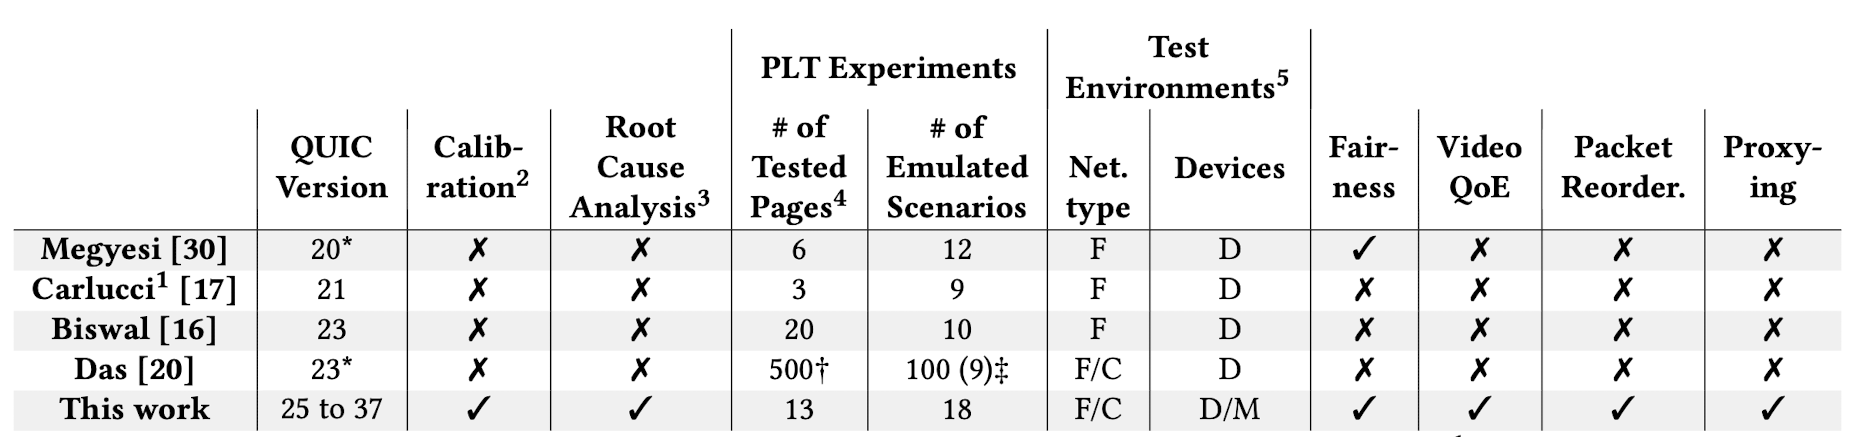
\includegraphics[width=\textwidth]{images/Kakhki overview.png}}
\caption{Comparison of experiments in \cite{Kakhki} to earlier papers}
\label{fig:Kakhki Comparison}
\end{figure*}

\subsection{Parameters}

\begin{table}
\begin{center}
\begin{tabular}{|c|c|}
\hline
\textbf{Parameter} & \textbf{Value ranges} \\
\hline
Bandwidth & 5Mbps - 200Mbps\\
Delay & 0ms - 100ms \\
Packet loss & 0\%, 1\%, 2\% \\
Object size & Small, large (often not specified in more detail) \\
Number of objects & 1 - 200 \\
\hline
\end{tabular}
\end{center}
\caption{Link parameters used in QUIC benchmarks}
\label{fig:quic-parameters}
\end{table}

In the description of their experiments, all papers start with a description of the testing environment. They set up a server and a client, which can either be a desktop or a mobile device. Then they continue to describe the condition of the link between the two participants. All papers that were included in this research have investigated the influence of the link's bandwidth, delay (round trip time), and packet loss. 

Furthermore, they vary the type of resource that is retrieved, especially the number of objects and the size of the individual objects. While some websites include a large number of small assets, e.g., CSS and Javascript files, others also contain large images and video files.

The exact values looked at for each parameter varied by paper, but table \ref{fig:quic-parameters} tries to summarise the most popular value choices.


\subsection{Megyesi - How quick is QUIC \cite{HowQuickIsQuic}}

% Megyesi - How quick is QUIC?
Megyesi uses QUIC version 20 together with the Google servers and an emulated network link. They report that there is no clear winner between QUIC and HTTP. In detail, their results are:

\begin{itemize}
\item QUIC performs poorly under very high bandwidth when large amounts of data must be downloaded
\item HTTP is the fastest protocol in case of high speed, high packet loss, and a high number of large objects.
\item QUIC performs very well compared to the other two protocols under high RTT values especially when the bandwidth is low
\item HTTP/2 performs very poorly in high loss environments due to HOL blocking. QUIC does not suffer as much.
\item Small object size favors QUIC and HTTP/2 against HTTP/1 due to multiplexing
\end{itemize} 

As mentioned in section \ref{sec:Performance}, Kakhki explains the first two results with the conservative maximum windows sizes used in the quite old QUIC version 20 used by Megyesi.

\begin{figure*}[htbp]
\centerline{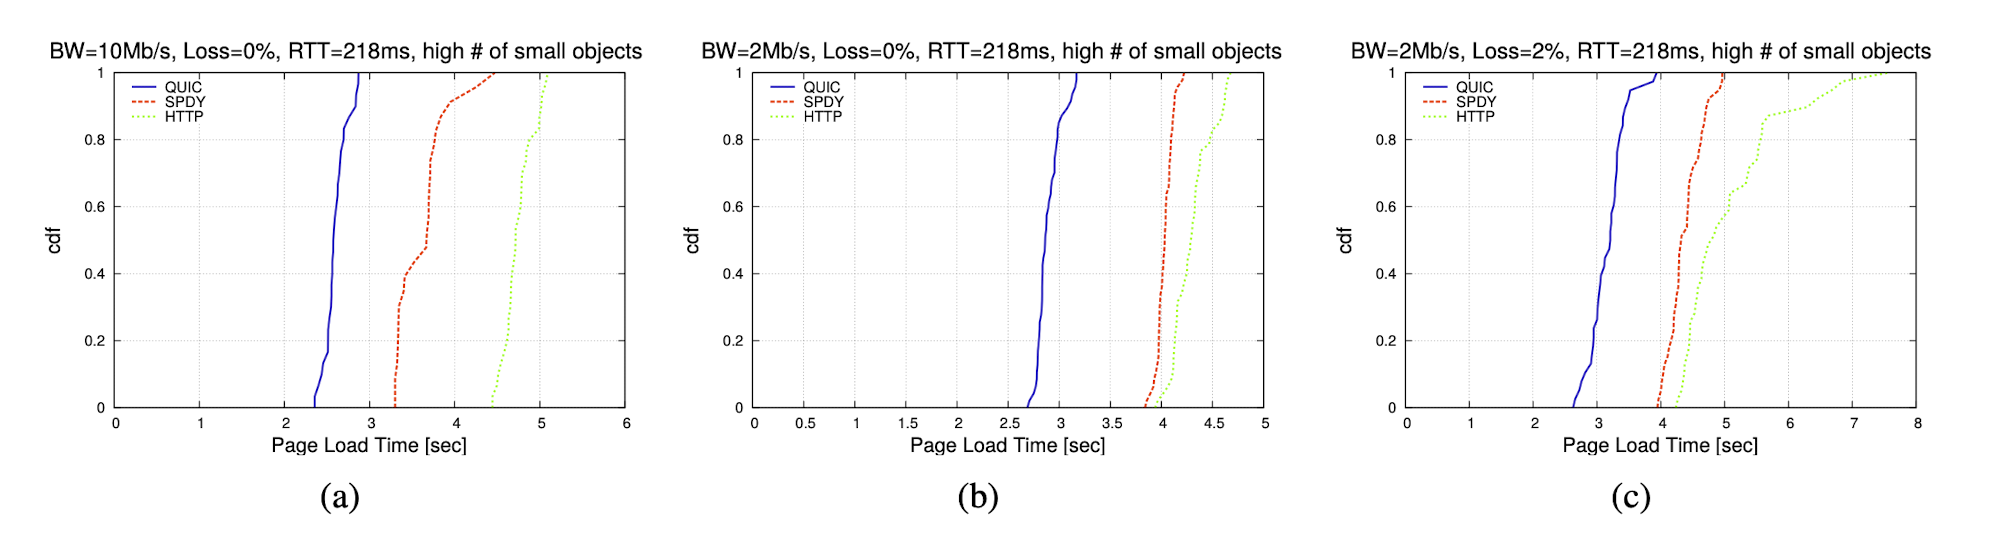
\includegraphics[width=\textwidth]{images/Megyesi QUIC wins.png}}
\caption{Scenarios in which QUIC outperforms HTTP/2 and HTTP/1 according to Megyesi \cite{HowQuickIsQuic}}
\label{fig:megyesi-quic-wins}
\end{figure*} 

\subsection{Nepomuceno - QUIC and TCP: A Performance Evaluation}

Nepomuceno \cite{Nepomuceno} measured the Page Load Times (PLT) of QUIC. They describe their methodology of finding a collection of 100 websites that have the same object distribution as the top ten thousand websites according to the Alexa site ranking \cite{AlexaRanking}. After finding their collection, they used a tool called Mahimahi to replay the websites under twelve different network conditions. They did not specify their QUIC version but instead specified their client as Google Chrome version 54. According to \cite{ChromeVersionHistory}, this version was released in October 2016 and, therefore, likely includes a QUIC version in the low 20s which is also rather old.

Table \ref{table:nepomuceno-results} shows the results of their investigation. The results are rather surprising given that there was no scenario in which QUIC outperformed TCP. 

They run their experiments twice with cache disabled in the first round and cache enabled in the second. The reason for that is that a client does not know upfront if the server is able or willing to communicate over QUIC. Therefore, Chrome starts the first connection with a server using TCP, and if the server replies with a certain header, the communication will be switched over to QUIC. Unfortunately, this behavior disables the 0RTT feature of QUIC which allows it to start a lot faster than TCP.

In the second round, they enabled the cache which would allow the client to remember if the server can use QUIC. In contrast to the expected increase in QUIC performance, TCP extends its lead even more. Nepomuceno does not investigate possible explanations for this behavior. According to their measurements, reading the answers from the server took significantly longer for QUIC than it did for TCP. They speculate that this is most likely due to the lacking optimizations of the QUIC stack.

Nevertheless, he notes that during the TCP experiments the client spent most of the time in the \textit{Connect Phase}. This underlines the fact that QUIC can start streams a lot faster than TCP. As later papers like \cite{Kakhki} and \cite{Kernel} have shown, the disadvantages of QUIC present at the time when Nepomuceno released his paper can be remedied with a more mature QUIC stack and optimized connection parameters for QUIC.

\begin{table}
\begin{center}
\begin{tabular}{|cc|cc|cc|}
\hline

\multicolumn{2}{|c|}{\textbf{Configuration}} & 
\multicolumn{2}{|c|}{\textbf{onLoad}} & 
\multicolumn{2}{|c|}{\textbf{onContentLoad}} \\
\hline

RTT & Package loss & CE & CD & CE & CD \\
\hline

20ms  & 0\%   & 17.24\% & 35.16\% & 9.67\%  & 34.37\% \\
20ms  & 0.5\% & 22.98\% & 34.06\% & 12.90\% & 37.50\% \\
20ms  & 1\%   & 24.13\% & 34.06\% & 8.60\%  & 39.58\% \\
20ms  & 2\%   & 16.09\% & 35.16\% & 4.30\%  & 40.62\% \\
100ms & 0\%   & 25.28\% & 29.67\% & 11.82\% & 36.45\% \\
100ms & 0.5\% & 21.83\% & 35.16\% & 7.52\%  & 36.45\% \\
100ms & 1\%   & 27.58\% & 31.86\% & 10.75\% & 37.50\% \\
100ms & 2\%   & 26.43\% & 34.06\% & 10.75\% & 40.62\% \\
200ms & 0\%   & 20.68\% & 28.57\% & 5.37\%  & 33.33\% \\
200ms & 0.5\% & 24.13\% & 32.96\% & 8.60\%  & 28.12\% \\
200ms & 1\%   & 25.28\% & 35.16\% & 9.67\%  & 30.20\% \\
200ms & 2\%   & 32.18\% & 39.56\% & 9.67\%  & 36.45\% \\
\hline

\end{tabular}
\end{center}

\caption{Results from \cite{Nepomuceno}. It shows the percentage of websites in which QUIC outperformed TCP with cache enabled (CE) and cache disabled (CD)}
\label{table:nepomuceno-results}
\end{table}

\subsection{Carlucci - HTTP over UDP: an experimental investigation of QUIC}

Carlucci \cite{HTTPoverUDP} reports that QUIC underperforms when a website has many objects due to the limited number of six concurrent QUIC streams in their test bed. However, they do not investigate the root cause of this rather surprising result, especially since their HTTP/1 client was also restricted to six TCP connections. They also state that HTTP is the clear winner when multiple objects suffer from packet loss.

\subsection{Langley - The QUIC Transport Protocol: Design and Internet-scale Deployment}

This paper was published by Google to showcase their development and results from the deployment of QUIC. It is the only paper presented here that encompasses a large-scale test run outside a controlled testing environment.

% Google Search latency
While Google has a vast amount of data centers that are connected over a private network, some of the Google servers are located in the networks of internet service providers. These servers are referred to as \textit{restricted edge locations (RELs)}. For various reasons, the RELs do not terminate TLS sessions. However, the TCP connection is terminated at the RELs to improve latency. The payload is then forwarded to a server within the Google network where the TLS session is terminated. \cite{Google}

In contrast, QUIC does not allow the termination of the transport session independently of the cryptographic session. Therefore, the RELs only proxy the QUIC connection. Nevertheless, QUIC was still able to improve the latency for Google searches compared to TCP by over 7\%. 

% Kakhki
% \subsection{Kakhki - Taking a Long Look at QUIC}

\subsection{Yu - Dissecting Performance of Production QUIC}

All of the papers that were already mentioned did not have to choose a QUIC implementation. At their release dates, only the open-source implementation of QUIC by Google was released as part of the Chromium project. Due to Google being the author of this implementation, many authors refer to this implementation as gQUIC. However, after the RFC 9000 was published that standardized QUIC, many other implementations saw the light of day. Yu was one of the researchers who published a more recent paper that compares different QUIC clients and servers and comes to a different conclusion \cite{Yu2}. 

Yu compared three clients against the endpoints of Google, Facebook, and Cloudflare, all of which have deployed QUIC for their public endpoints. They found endpoints that serve static data in various sizes and used them to compare the three vendors. While earlier papers often tried to remove the variability that comes from using public endpoints, Yu purposefully chose to use them to test different proprietary deployments and different configurations of QUIC servers. In addition to that, they used three different HTTP/3 clients against each endpoint to look for edge cases. The variety of clients and servers also allows them to test if a performance benefit comes from a specific implementation of QUIC, or the design of QUIC itself.

The first benchmark encompasses the retrieval of a single static object of varying size. For each combination of client, server, and object, the time to last byte (TTLB) was measured. They showed, that QUIC performed consistently better than HTTP/2 for smaller payloads without added loss or delay. This behavior was the same regardless of the client or server and is, therefore, likely a result of the design of QUIC. They attribute this advantage to the 1RTT mechanism of QUIC, which has a bigger impact when the connections are short-lived. For larger payloads, HTTP/3 performed similarly to HTTP/2.

\begin{figure}[htbp]
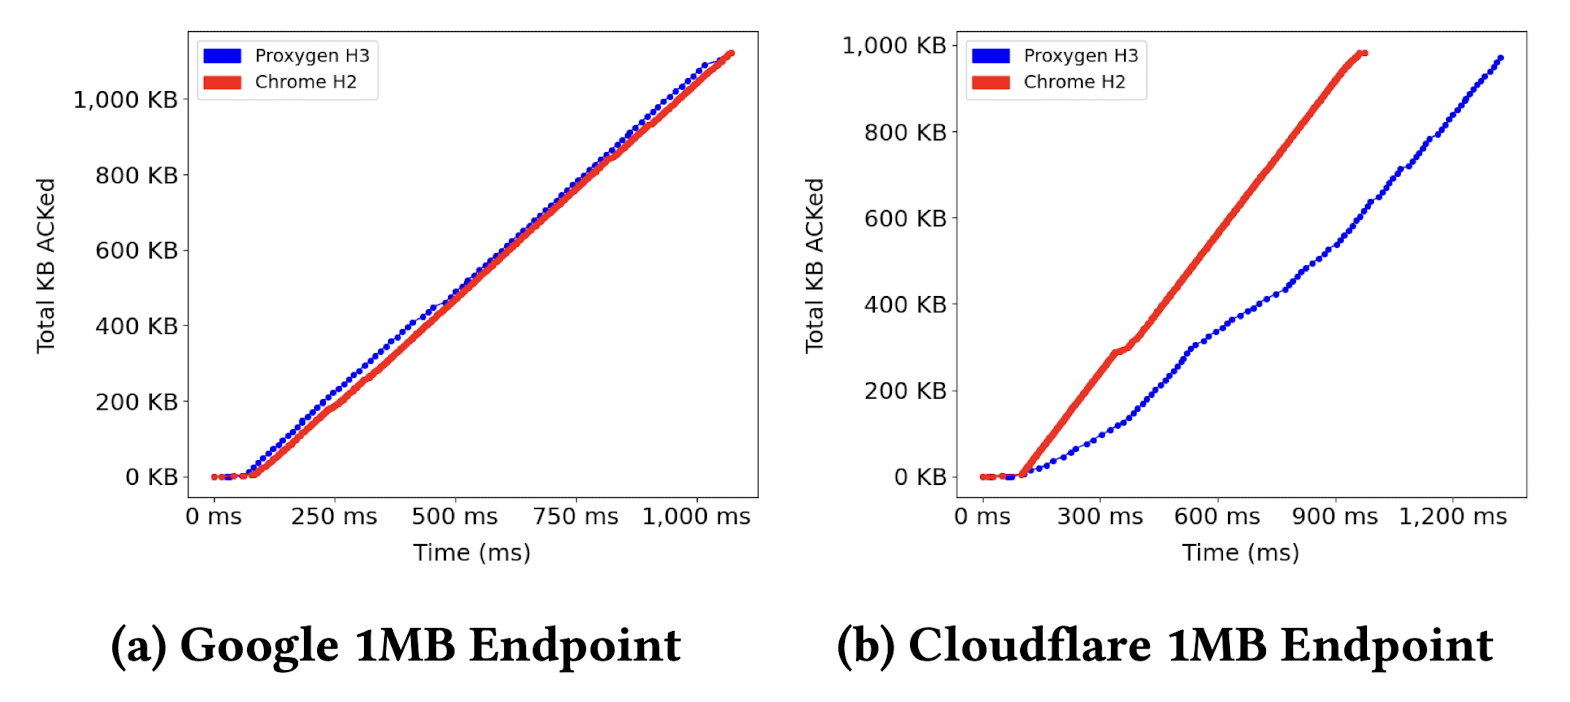
\includegraphics[width=8cm,keepaspectratio]{images/Yu2/Cloudflare anomaly.png}
\caption{Bytes acknowledged for 1MB payloads with 1\% loss \cite{Yu2}}
\label{fig:yu2-cloudflare-anomaly}
\end{figure}

\begin{figure*}[h]
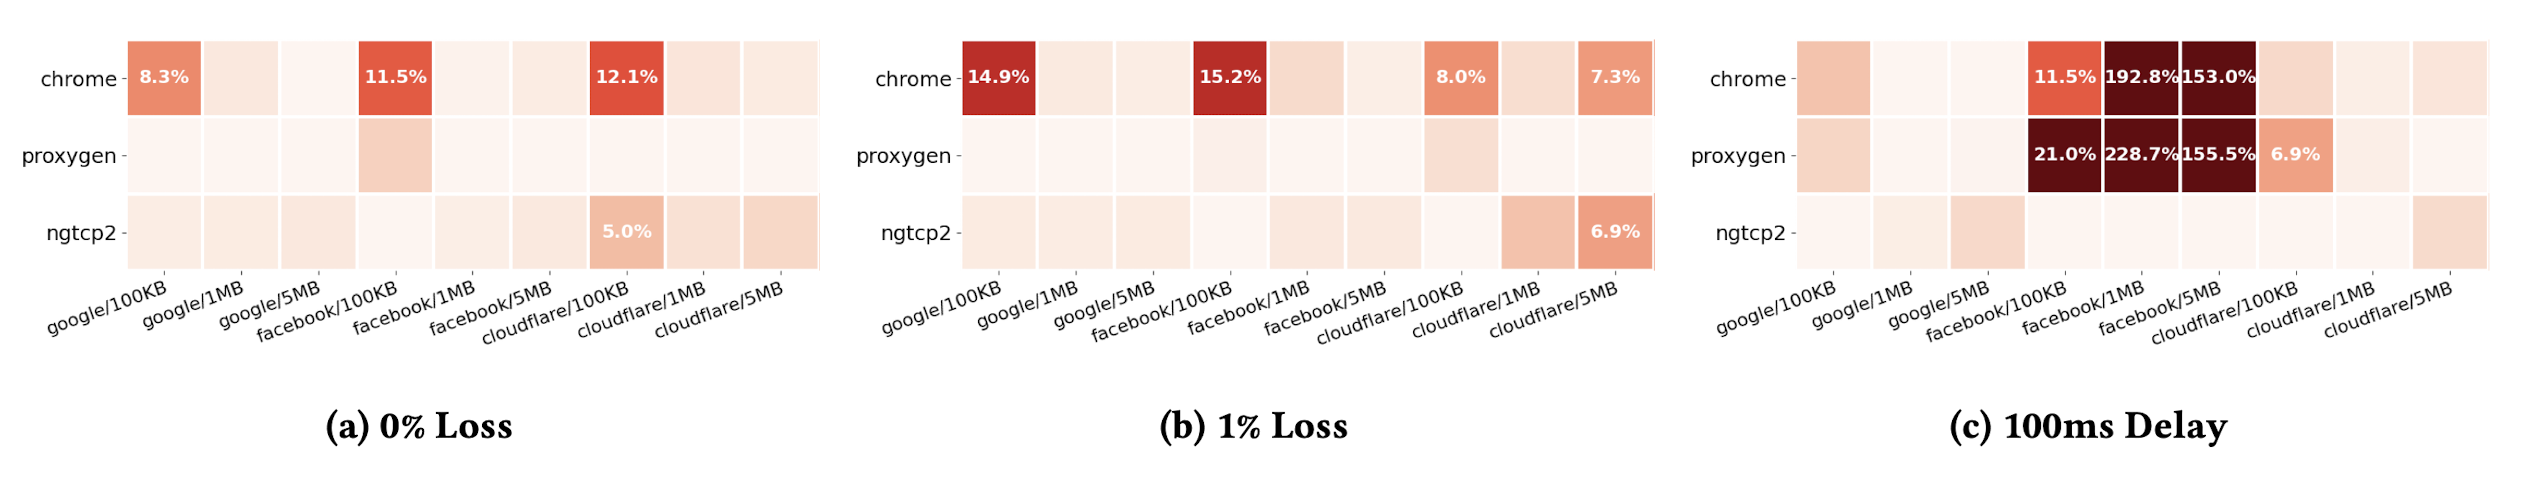
\includegraphics[width=\textwidth,keepaspectratio]{images/Yu2/HTTP3 Single object benchmarks.png}
\caption{Heatmaps from \cite{Yu2} that show the performance differences between HTTP/3 clients. Each cell shows the difference from the median TTLB to the lowest TTLB of any client. Therefore, 0\% is the best value that can be achieved. Differences below 5\% are not labelled.}
\label{fig:yu2-http3-single-object-benchmark}
\end{figure*}

After that, Yu added extra loss to the connection. Similar to the first test, HTTP/3 performed better for smaller payloads of 100KB in size, while HTTP/2 caught up to HTTP/3 for bigger payloads. However, only for the Cloudflare endpoint, HTTP/3 performed notably worse as seen in figure \ref{fig:yu2-cloudflare-anomaly}. This anomaly was caused by the differing congestion control algorithms. Cloudflare uses Cubic for QUIC, but BRR for TCP. Cubic uses packet loss for congestion control and sets the maximum sending window to the current windows when a packet is lost. In contrast, BBR uses the rate of ACK packets sent back from the receiver and, hence, can utilize the full bandwidth of a link better in the presence of extra loss. This result shows that QUIC's feature of pluggable congestion control algorithms necessitates the differentiation between QUIC itself and the congestion control used. Otherwise, researchers might come to false conclusions about QUIC itself. Furthermore, it shows that vendors might need to adapt their congestion control to the condition of the network links they expect users to use.

When Yu performs another round of his experiments with added delay to increase the RTT, they noticed another anomaly. QUIC outperformed HTTP/2 substantially due to the decrease in required round trips to establish a connection. However, for the endpoints provided by Facebook, the QUIC-enabled HTTP client Proxygen \cite{Proxygen}, published by Facebook itself, performed tremendously badly as shown in figure \ref{fig:yu2-http3-single-object-benchmark}. After some investigation, Yu found out that this behavior was caused by a bug in the BBR implementation of Proxygen. Again, this bug underlines that the chosen implementation of QUIC can have more effect on the results of experiments than the design of QUIC itself.

\begin{figure}[htbp]
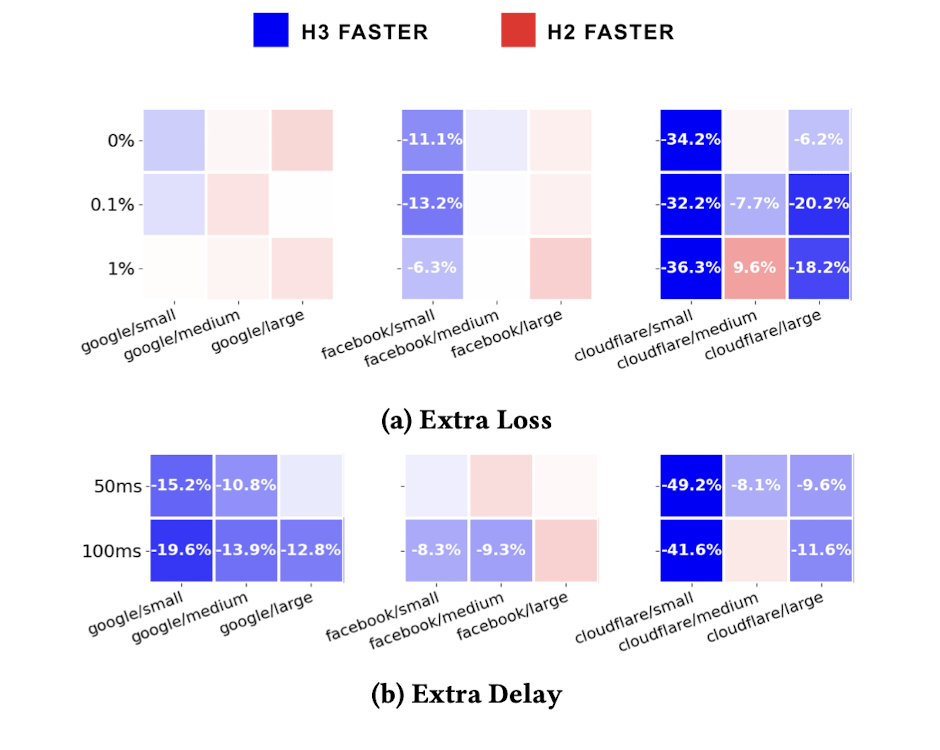
\includegraphics[width=8cm,keepaspectratio]{images/Yu2/HTTP3 Multiple objects benchmark.png}
\caption{HTTP/3 vs HTTP/2 performance based on SI. The speed of the network link was 10Mbps.}
\label{fig:yu2-http3-multiple-object-benchmark}
\end{figure}

After testing the performance of HTTP/3 with single objects, Yu proceeded to test real websites with multiple objects. All multi-object tests were measured using a metric called Speed Index (SI) which describes how much the screen space visible to the user changes during loading. A low SI score describes a website that loads instantly rather than gradually. Hence, a low SI score is preferred.

HTTP/3 removes the HOL blocking present in HTTP/2. Because of this, someone would expect the results to be in favor of HTTP/3 when more loss is added to the link for Facebook and Google, but not for Cloudflare due to the aforementioned usage of Cubic. Furthermore, HTTP/2 and HTTP/3 are both stream-native protocols and due to the fewer roundtrips of QUIC, it is also to be expected that HTTP/3 has an edge over HTTP/2 for smaller websites as it can start to stream faster.

While the results of the multi-object test, shown in figure \ref{fig:yu2-http3-multiple-object-benchmark}, show the advantage of HTTP/3 for smaller payloads again, they also reject the hypothesis that the removal of HOL blocking makes it more resilient to additional loss. For both Facebook and Google, the difference in the medium and large websites was negligible. 

\begin{figure}[htbp]
  \begin{center}
  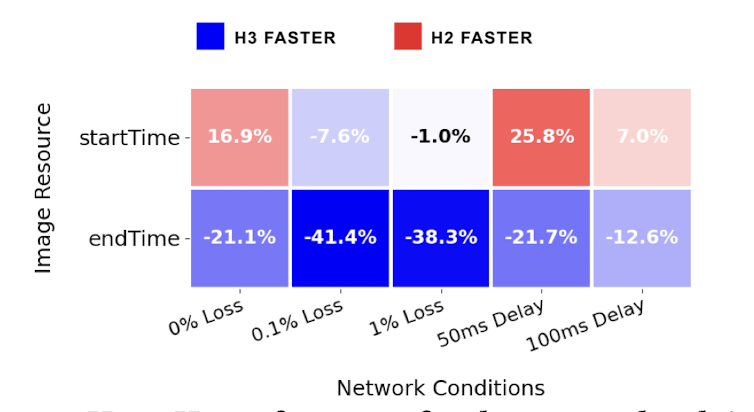
\includegraphics[width=8cm,keepaspectratio]{images/Yu2/Image load comparison.png}
  \caption{Start and end times for loading the image on the large Cloudflare website with HTTP/2 and HTTP/3}
  \label{fig:yu2-image-load-comparison}
  \end{center}
\end{figure}

\begin{figure}[htbp]
  \begin{center}
  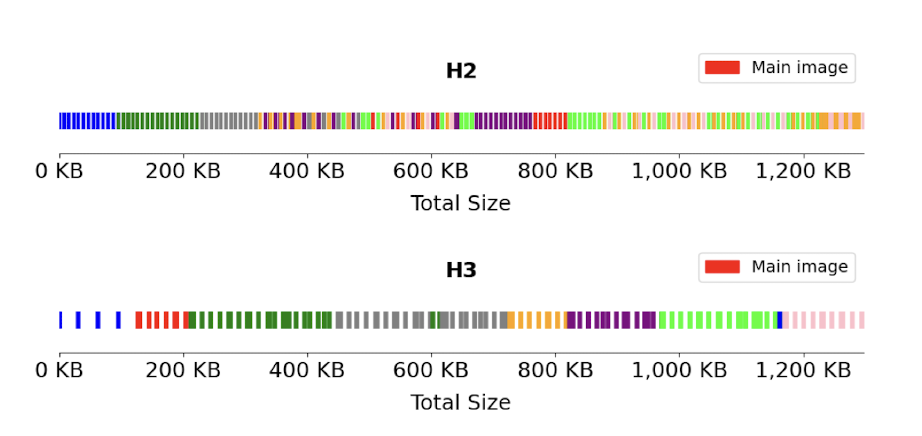
\includegraphics[width=8cm,keepaspectratio]{images/Yu2/Chrome HTTP frames.png}
  \caption{HTTP frames received by Chrome for the large Cloudflare website}
  \label{fig:yu2-chrome-http-frames}
  \end{center}
\end{figure}

Contrary to the expectations, Cloudflare scores were undoubtedly in favor of HTTP/3 with added loss or added delay even for the medium and large websites. The large website contains a large image at the center of the initial screen presented to the user. HTTP/3 was able to load this image faster which resulted in a lower SI score. The extracted HAR logs from Google Chrome, visualized in figure \ref{fig:yu2-image-load-comparison}, show that H3 was able to load the image a lot faster even if requested later. 

Yu states that Chrome has assigned similar priorities to the objects of the website when using either HTTP/2 or HTTP/3, prioritizing the main image over other resources. Figure \ref{fig:yu2-chrome-http-frames} shows that Chrome received the main image in one chunk at the beginning of the connection when HTTP/3 was used. However, over the HTTP/2 connection, Chrome received the image a lot later. 

Once again, this result comes from an implementation detail rather than the protocol design. A Cloudflare engineer confirmed to Yu that Cloudflare decided to ignore the browser-based prioritization for images in HTTP/2, which, according to them, should improve performance. Furthermore, the engineer also disclosed that Cloudflare also ignores the priorities in HTTP/3. However, in the latter case, the FIFO scheduler of Cloudflare just so happened to send the image first.

\begin{figure}[htbp]
  \begin{center}
  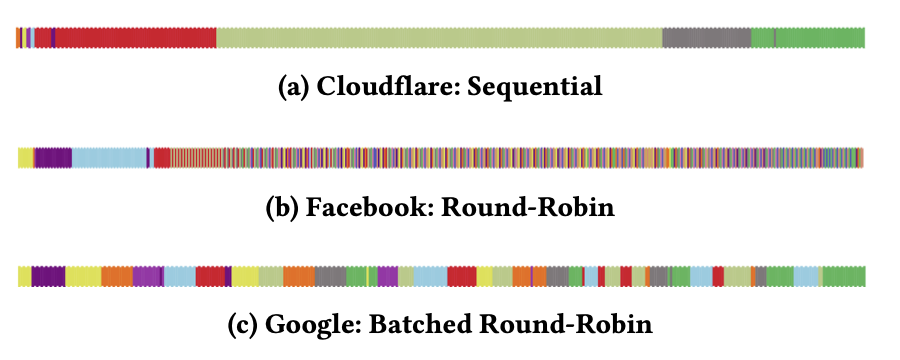
\includegraphics[width=8cm,keepaspectratio]{images/Yu2/HTTP3 multiplexing strategies.png}
  \caption{HTTP frames received by Chrome for the large Cloudflare website}
  \label{fig:yu2-multiplexing-strategies}
  \end{center}
\end{figure}

However, this does not explain why the image was sent without any interruption from other objects. While QUIC supports the multiplexing of multiple streams over a single connection with priorities assigned to each stream, it does not specify how the data should be sent back to the client. This is an implementation detail that is up to the deployment of the server. Figure \ref{fig:yu2-multiplexing-strategies} shows the different strategies used by the vendors that Yu investigated. Cloudflare's usage of sequential transfer means that the streams are not multiplexed in parallel at all. This is another instance where researchers have to look not only in the RFC for QUIC to determine its inner working but have to check how different vendors handle the same situation differently.

\section{Conclusion}

In this paper, we compared the performance results of different researchers who benchmarked QUIC and HTTP/3 and compared the results to either HTTP/1, HTTP/2, or both. We show that due to the rapid development of QUIC in the last years, it is crucial to know the year and exact QUIC version a researcher has used to conduct the experiments.

Earlier papers published before the QUIC RFC was finalized solely focused on the open-source implementation provided by Google. Their results were mixed but could mostly agree that QUIC performs well in network conditions that emulate a mobile connection: low bandwidth, high packet loss, and high delay. However, HTTP/1 outperformed it measurably when the link was more stable and bandwidth was high.

QUIC evolved and later versions were more tuned to perform well in the latter case. Kakhki \cite{Kakhki} and Yu \cite{Yu2} have shown that increasing the conservative configuration options used by earlier QUIC versions helps QUIC to perform better in high bandwidths environments. Furthermore, Yu has shown that performance measurements of QUIC must be treated with more care than benchmarks of the more mature TCP due to differences in the rather new QUIC implementations. 

Coming back to the topic of this paper, all papers cited in this work have shown that the 0RTT and 1RTT features of QUIC improve the startup times of QUIC. In all presented experiments, QUIC always had an edge on both HTTP/2 and HTTP/1 when the transmitted payload was small, as the savings of some round-trips compared to TCP are more significant when the connection is short-lived.

\bibliographystyle{plain}
\bibliography{references.bib}

\end{document}
